\section{Topology Design Anti-Patterns}
\label{sec:anti-pattern}
This elaborates on the anti-patterns we elicited through self-ethnography. These anti-patterns are elaborated further within OSTIA to allow for their detection during streaming topology inference analysis.

\subsection{Multi-Anchoring}
In order to guarantee fault-tolerant stream processing, tuples processed by bolts needs to be anchored with the unique id of the bolt and be passed to multiple acknowledgers (or ``ackers" in short) in the topology. In this way, ackers can keep track of tuples in the topology.\\
\emph{\bf TODO: what is the consequence of these anti-patterns? How does OSTIA detect?}

\begin{figure}[H]
	\begin{center}
		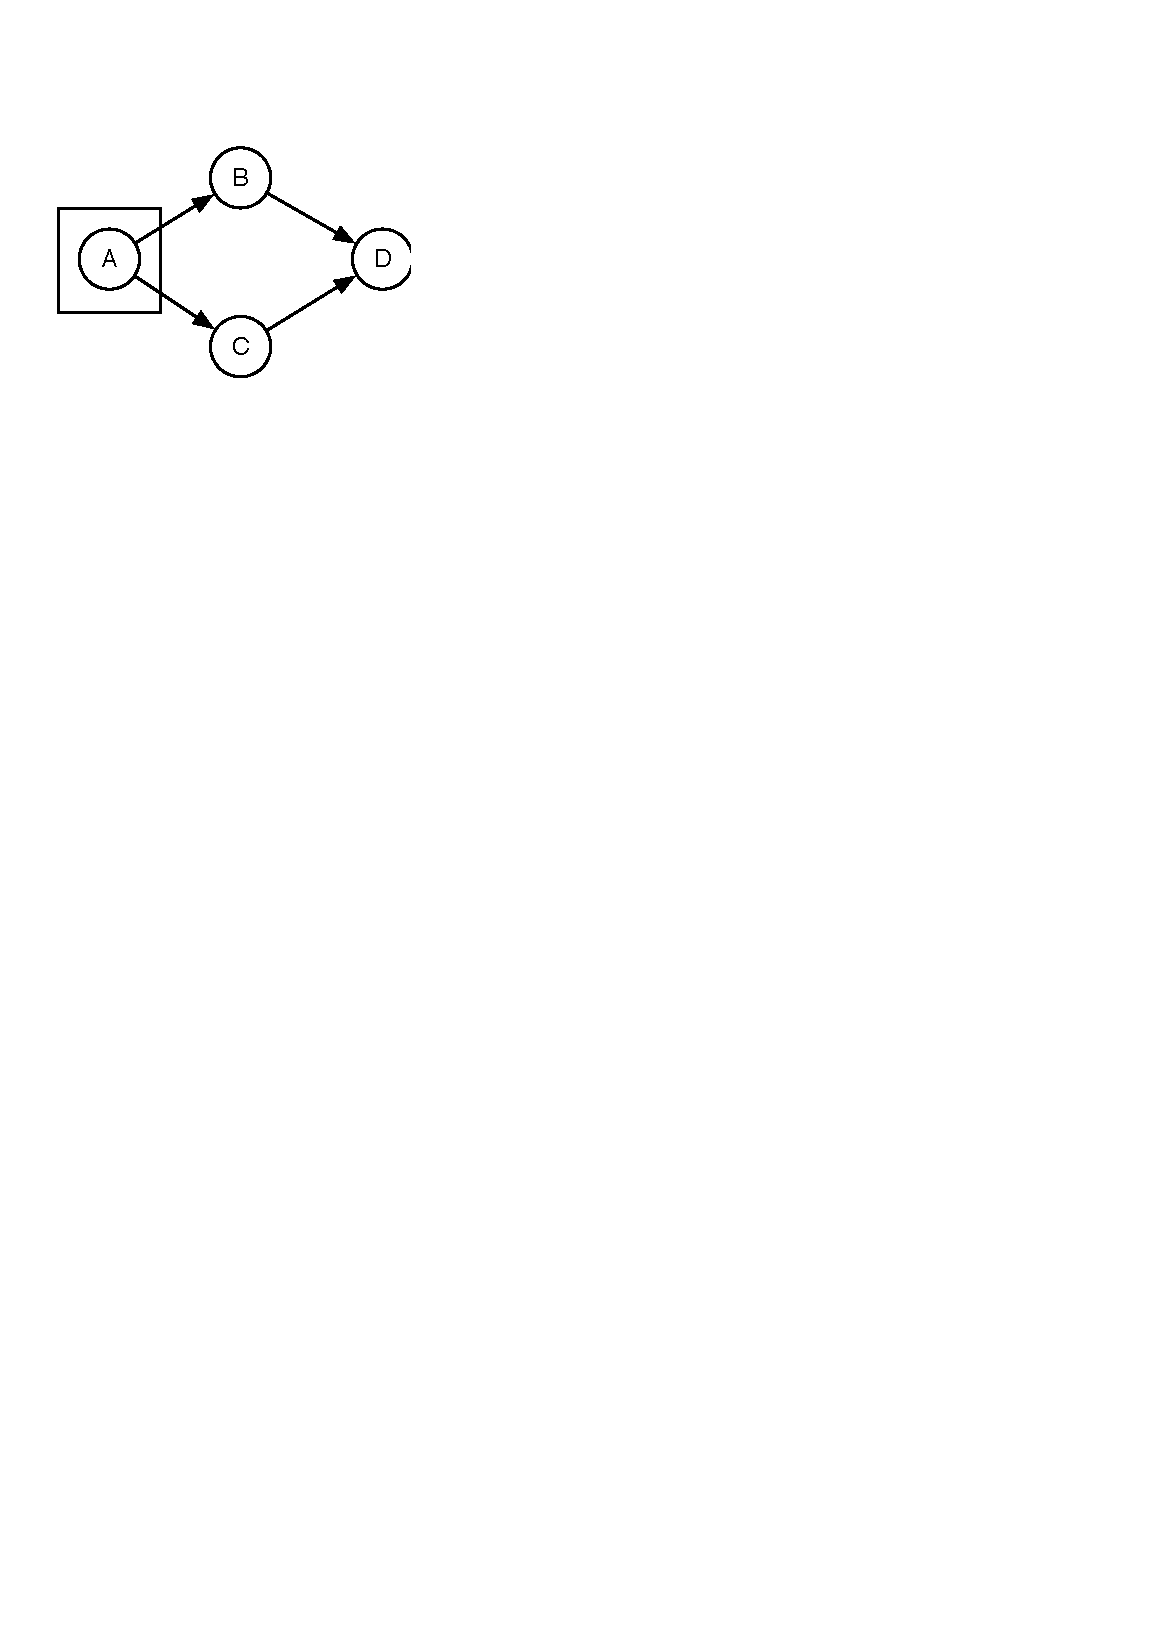
\includegraphics[width=4cm]{images/multi-anchoring}
		\caption{Multi-anchoring.}
		\label{fig:multi-anchoring}
	\end{center}
\end{figure}

\subsection{Cycle in Topology}

Technically it is possible to have cycle in Storm topologies. An infinite cycle of processing would create an infinite tuple tree and make it impossible for Storm to ever acknowledge spout emitted tuples. Therefore, cycles should be avoided or resulting tuple trees should be investigated additionally to make sure they terminate at some point and under a specified series of conditions.

\begin{figure}[H]
	\begin{center}
		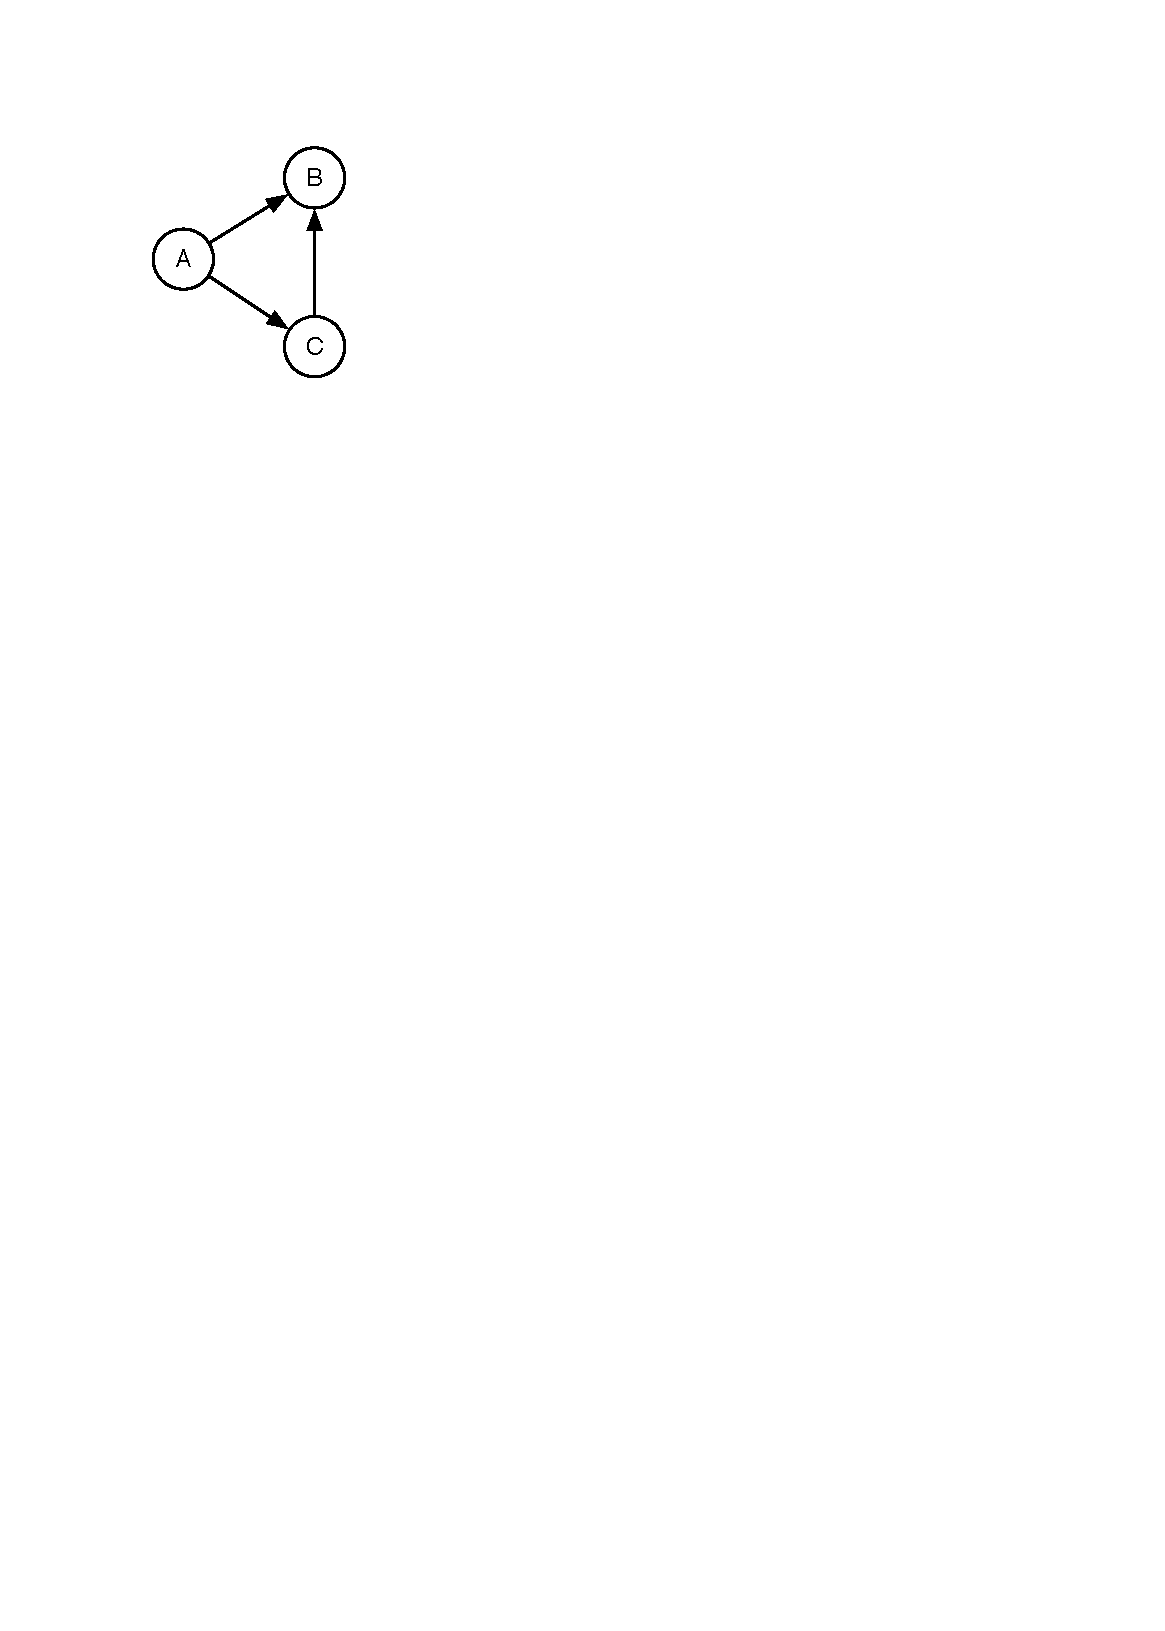
\includegraphics[width=3cm]{images/cycle}
		\caption{Cycle n Topology.}
		\label{fig:cycle}
	\end{center}
\end{figure}

\subsection{Persistent Data}

This pattern covers the circumstance wherefore if two processing elements need to update a same entity in a storage, there should be a consistency mechanism in place. 


\begin{figure}[H]
	\begin{center}
		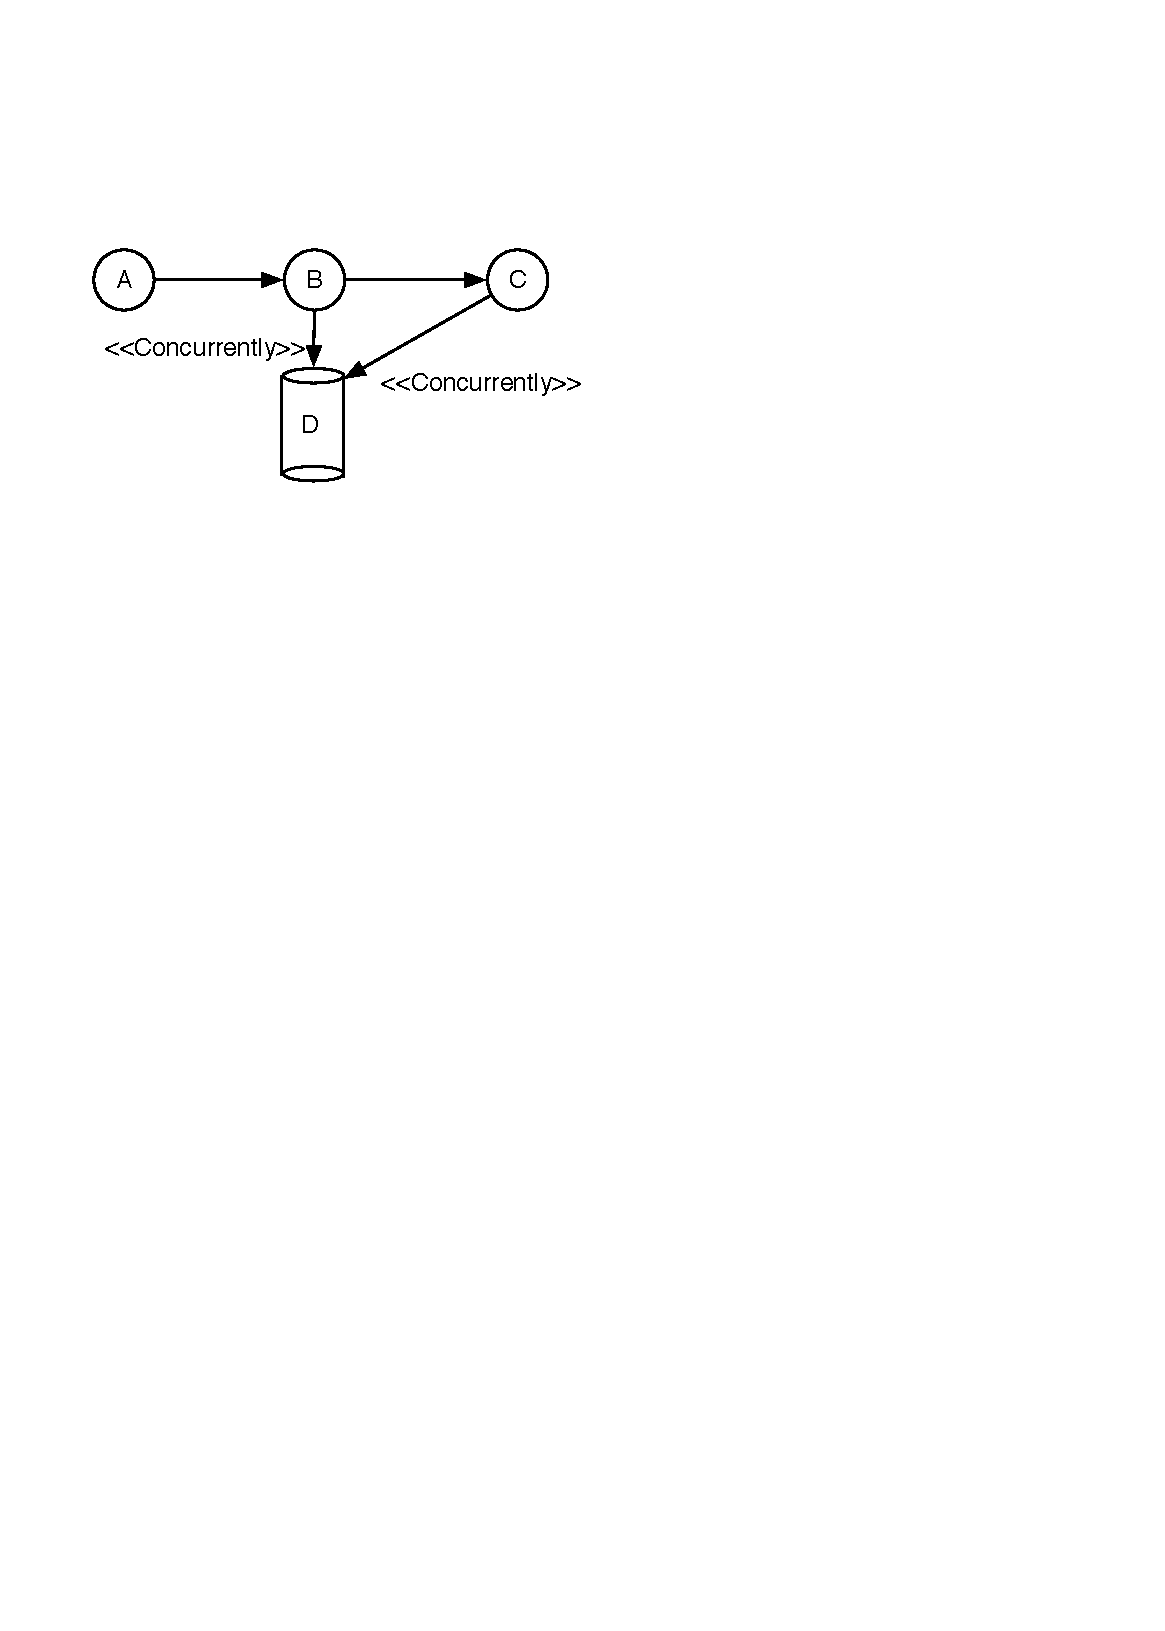
\includegraphics[width=4cm]{images/persistence}
		\caption{Concurrency management.}
		\label{fig:persistence}
	\end{center}
\end{figure}

\section{Algorithmic Analysis on Stream Topologies}\label{algo}

\subsection{fan-in/fan-out}

For Bolts, fan-in is the number of processing elements (Bolts and Spouts) that are connected to this specific bolt in the topology and fan-out is the number of PEs that are dependent to this specific bolt. For Spouts, fan-in is the number of topics (from the messaging broker, i.e., Apache Kafka for Storm) that this specific spout is subscribed to and fan out is the number of bolts that is dependent to this spout.

\begin{figure}[H]
	\begin{center}
		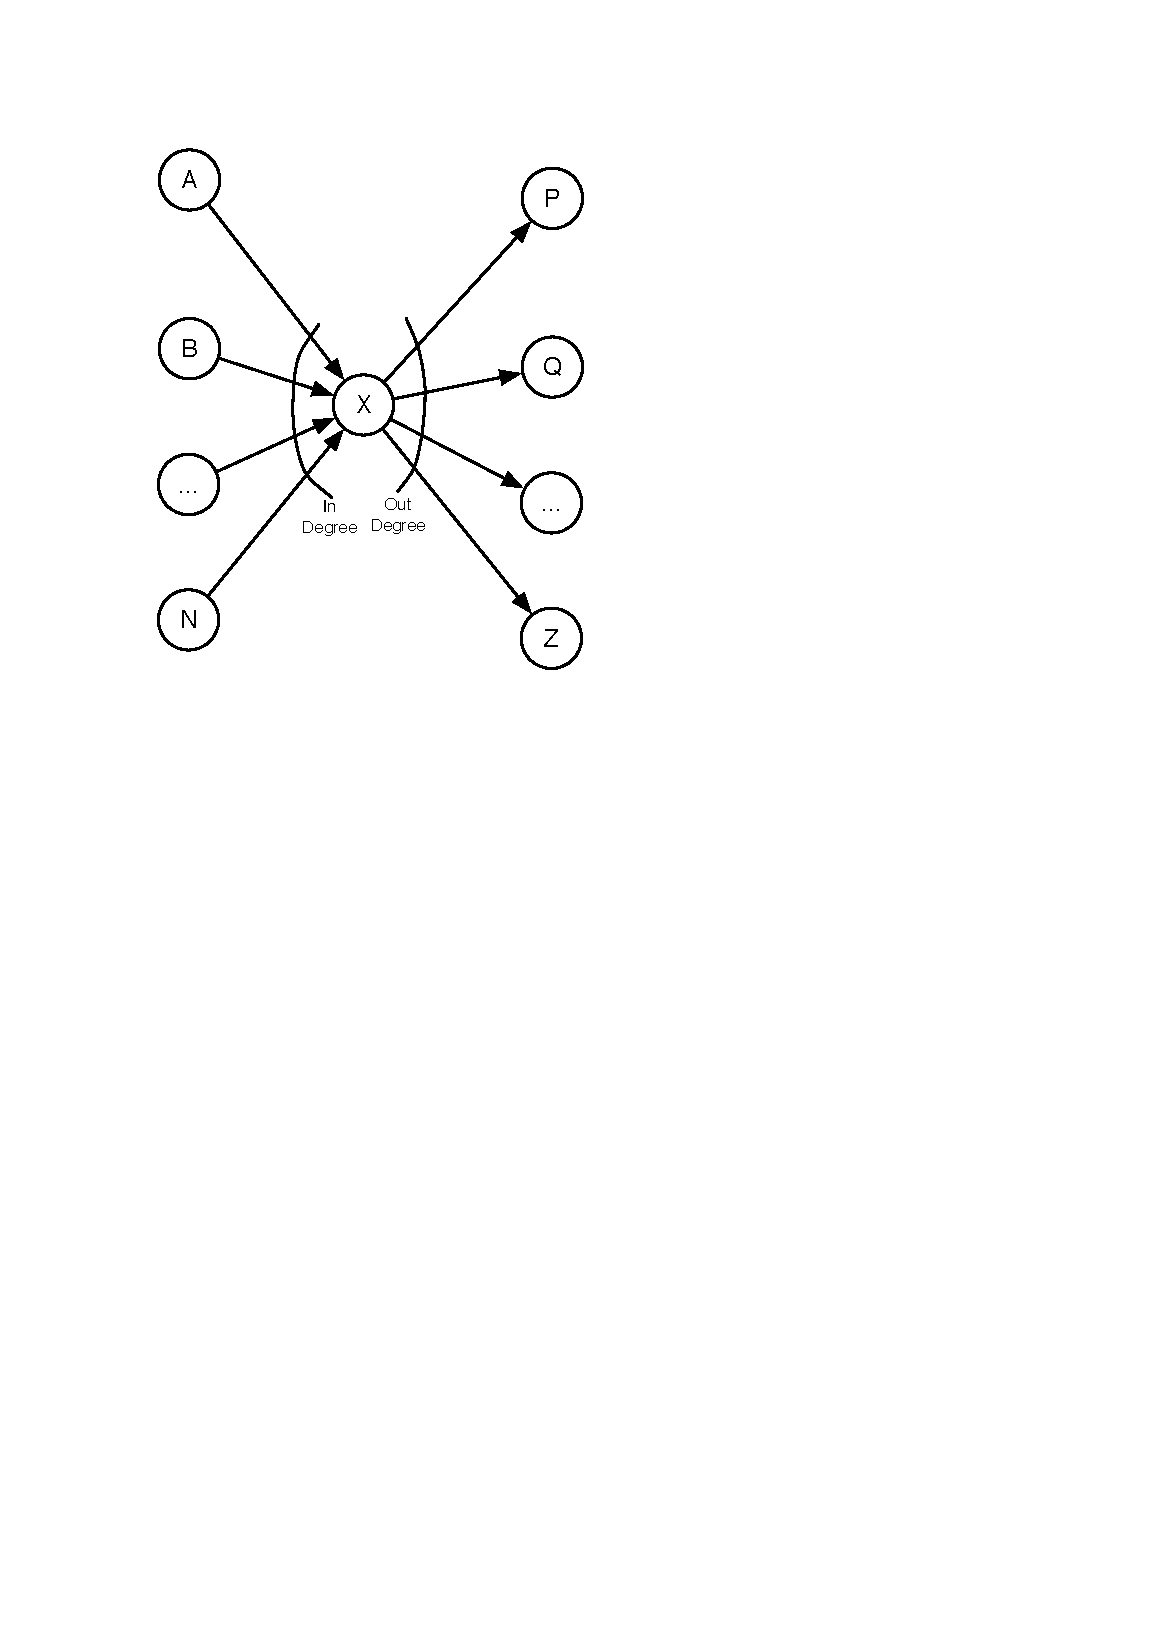
\includegraphics[width=3cm]{images/fan-in-out}
		\caption{Fan-in fan-out in Stream topologies.}
		\label{fig:fan}
	\end{center}
\end{figure}

\subsection{topology cascading}

By topology cascading, we mean connecting two different Storm topologies via a messaging framework (e.g., Apache Kafka). This circumstance, which is actually part of our evaluation and case-studies, may raise the complexity of the overarching topology to unacceptable levels and may require additional attention.

\begin{figure}[H]
	\begin{center}
		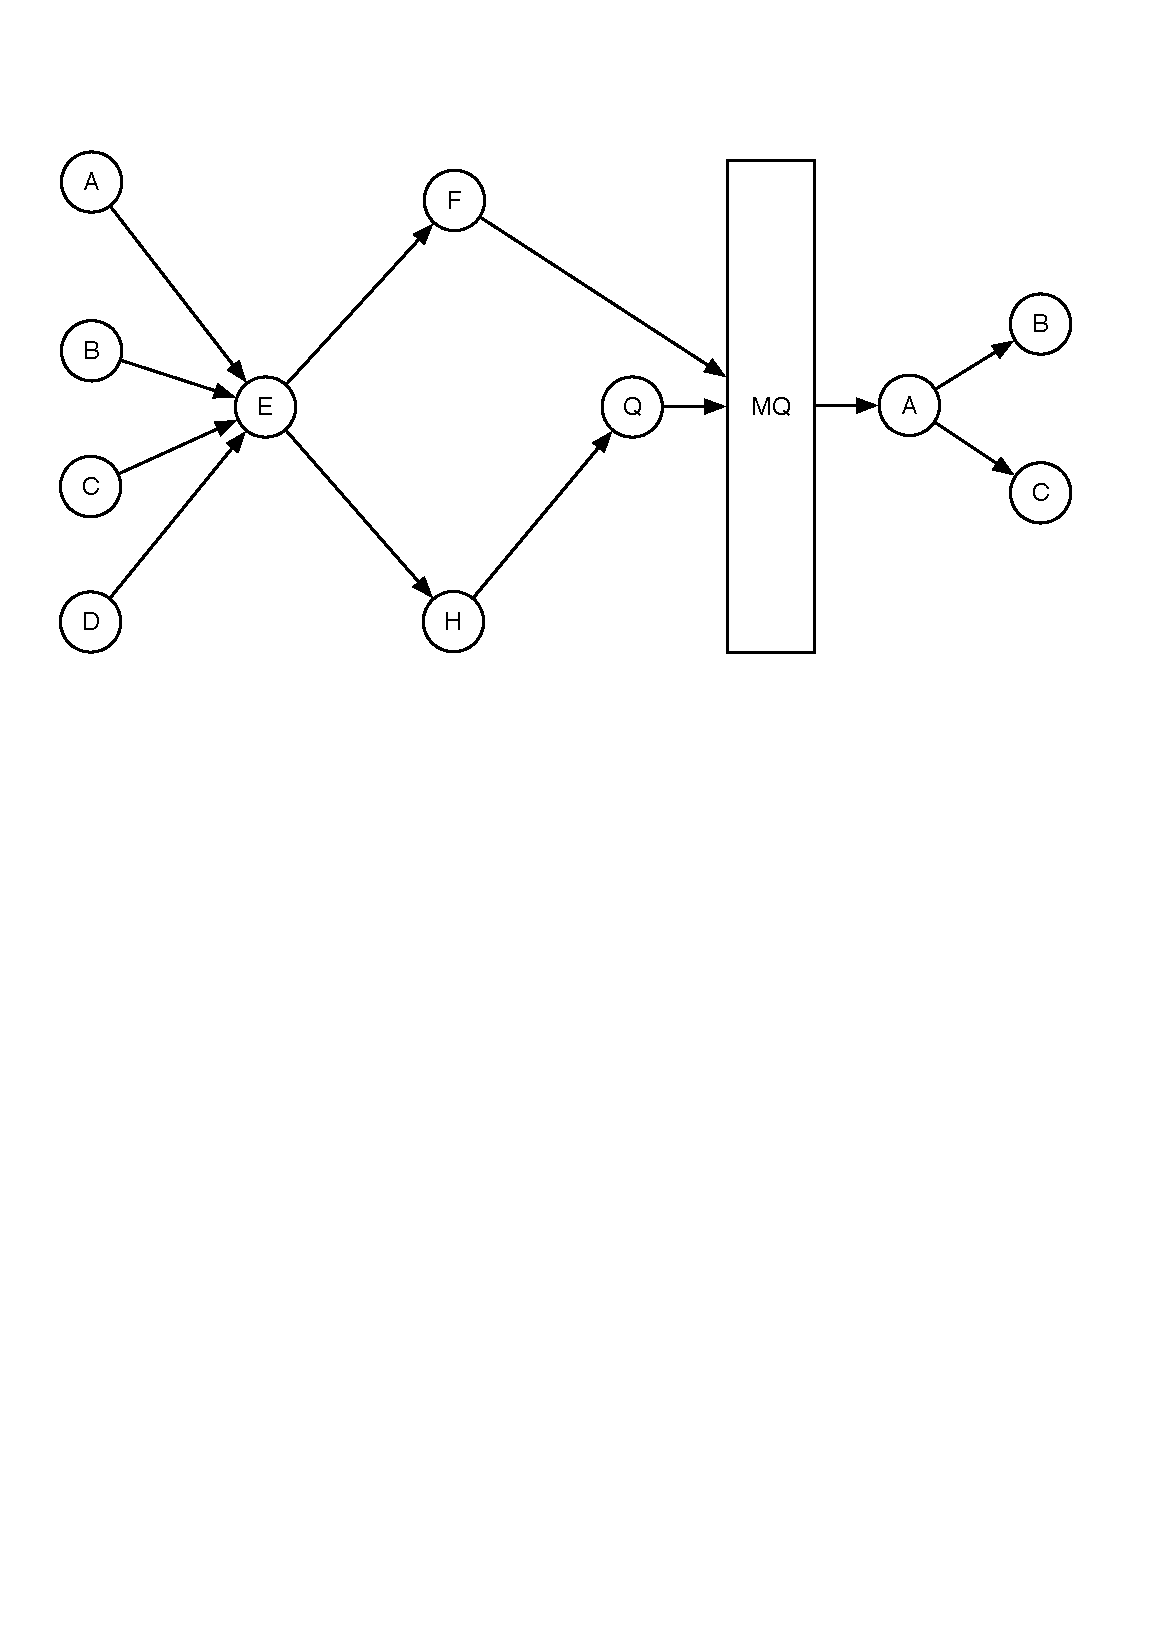
\includegraphics[width=5cm]{images/cascading}
		\caption{cascading.}
		\label{fig:cascading}
	\end{center}
\end{figure}

\subsection{Topology clustering}
Identifying the coupled processing elements and put the in a cluster in a way that elements in a cluster have high cohesion and less coupled with the elements in other clusters. Simple clustering or Social-Network Analysis mechanisms can be used to infer clusters. These clusters may require additional attention since they could turn out to become bottlenecks.

\begin{figure}[H]
	\begin{center}
		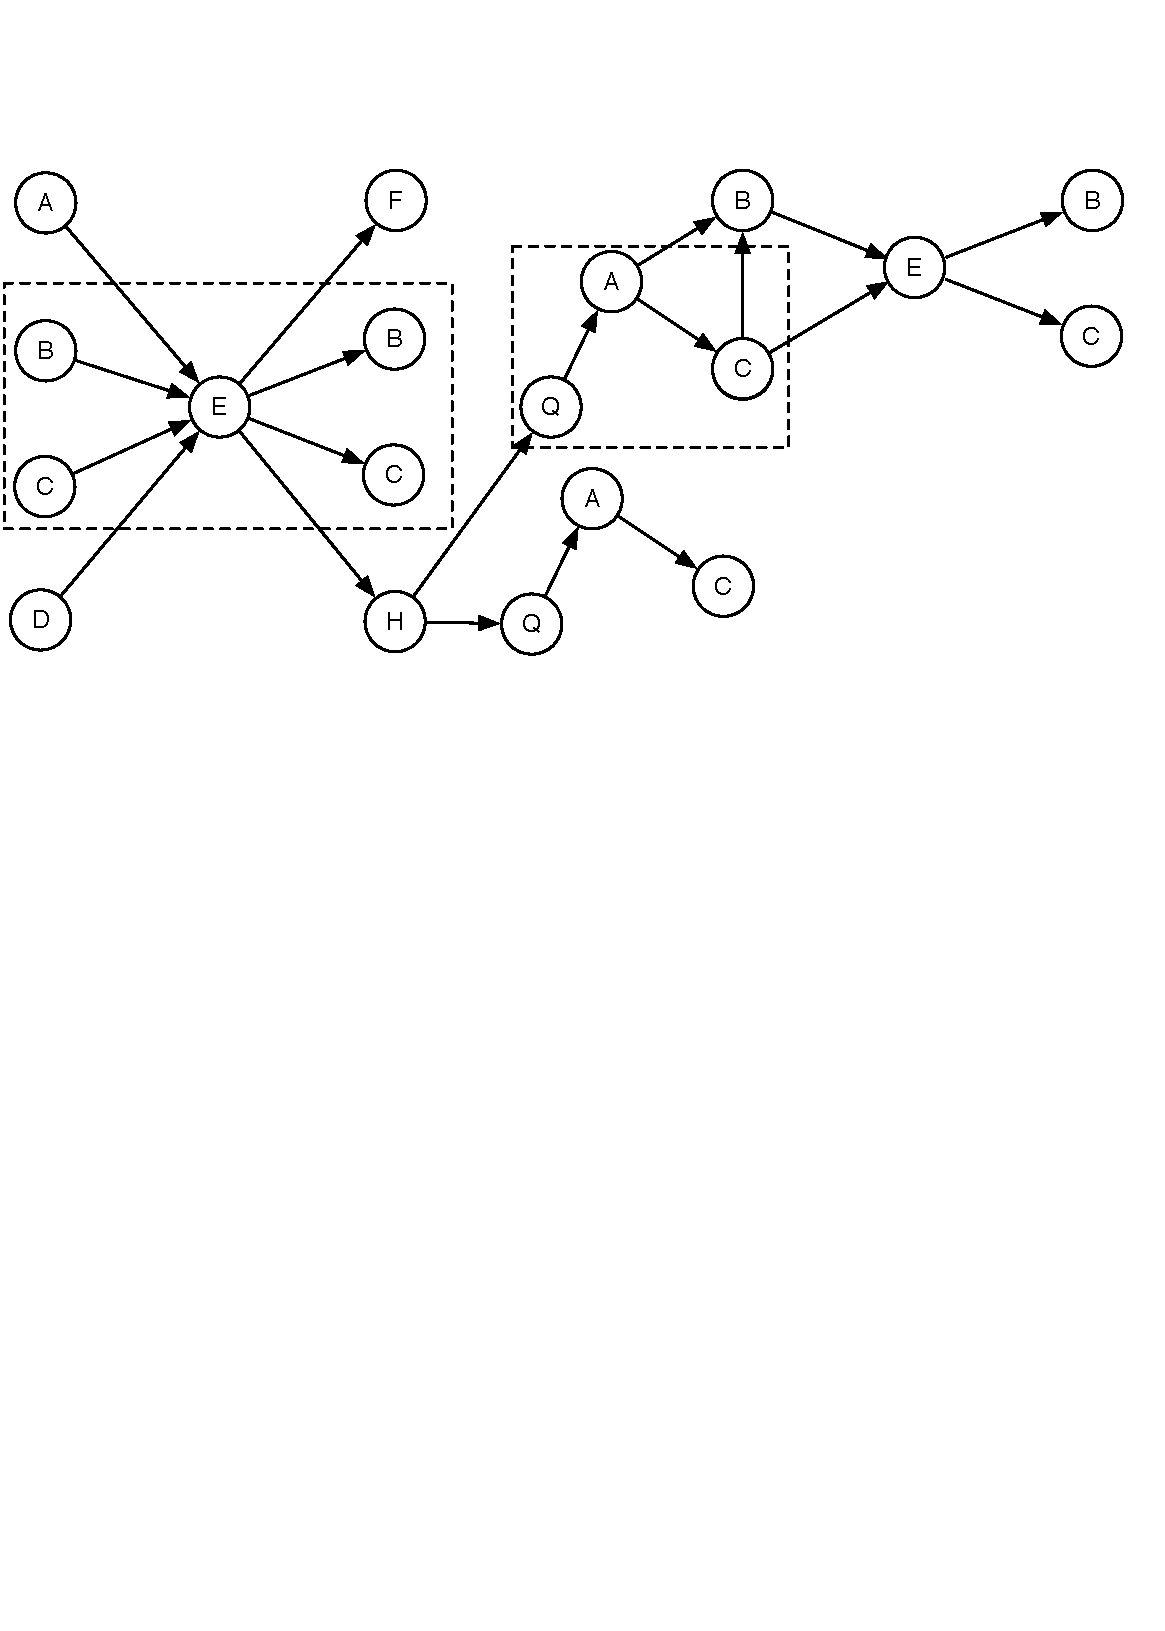
\includegraphics[width=5cm]{images/clustering}
		\caption{clustering.}
		\label{fig:clustering}
	\end{center}
\end{figure}

\subsection{Computation funnel}
A computational funnel emerges when there is not a path from data source (spout) to the bolts that sends out the tuples off the topology to another topology through a messaging framework or through a storage. This circumstance should be dealt with since it may compromise the availability of results under the desired performance restrictions.

\begin{figure}[H]
	\begin{center}
		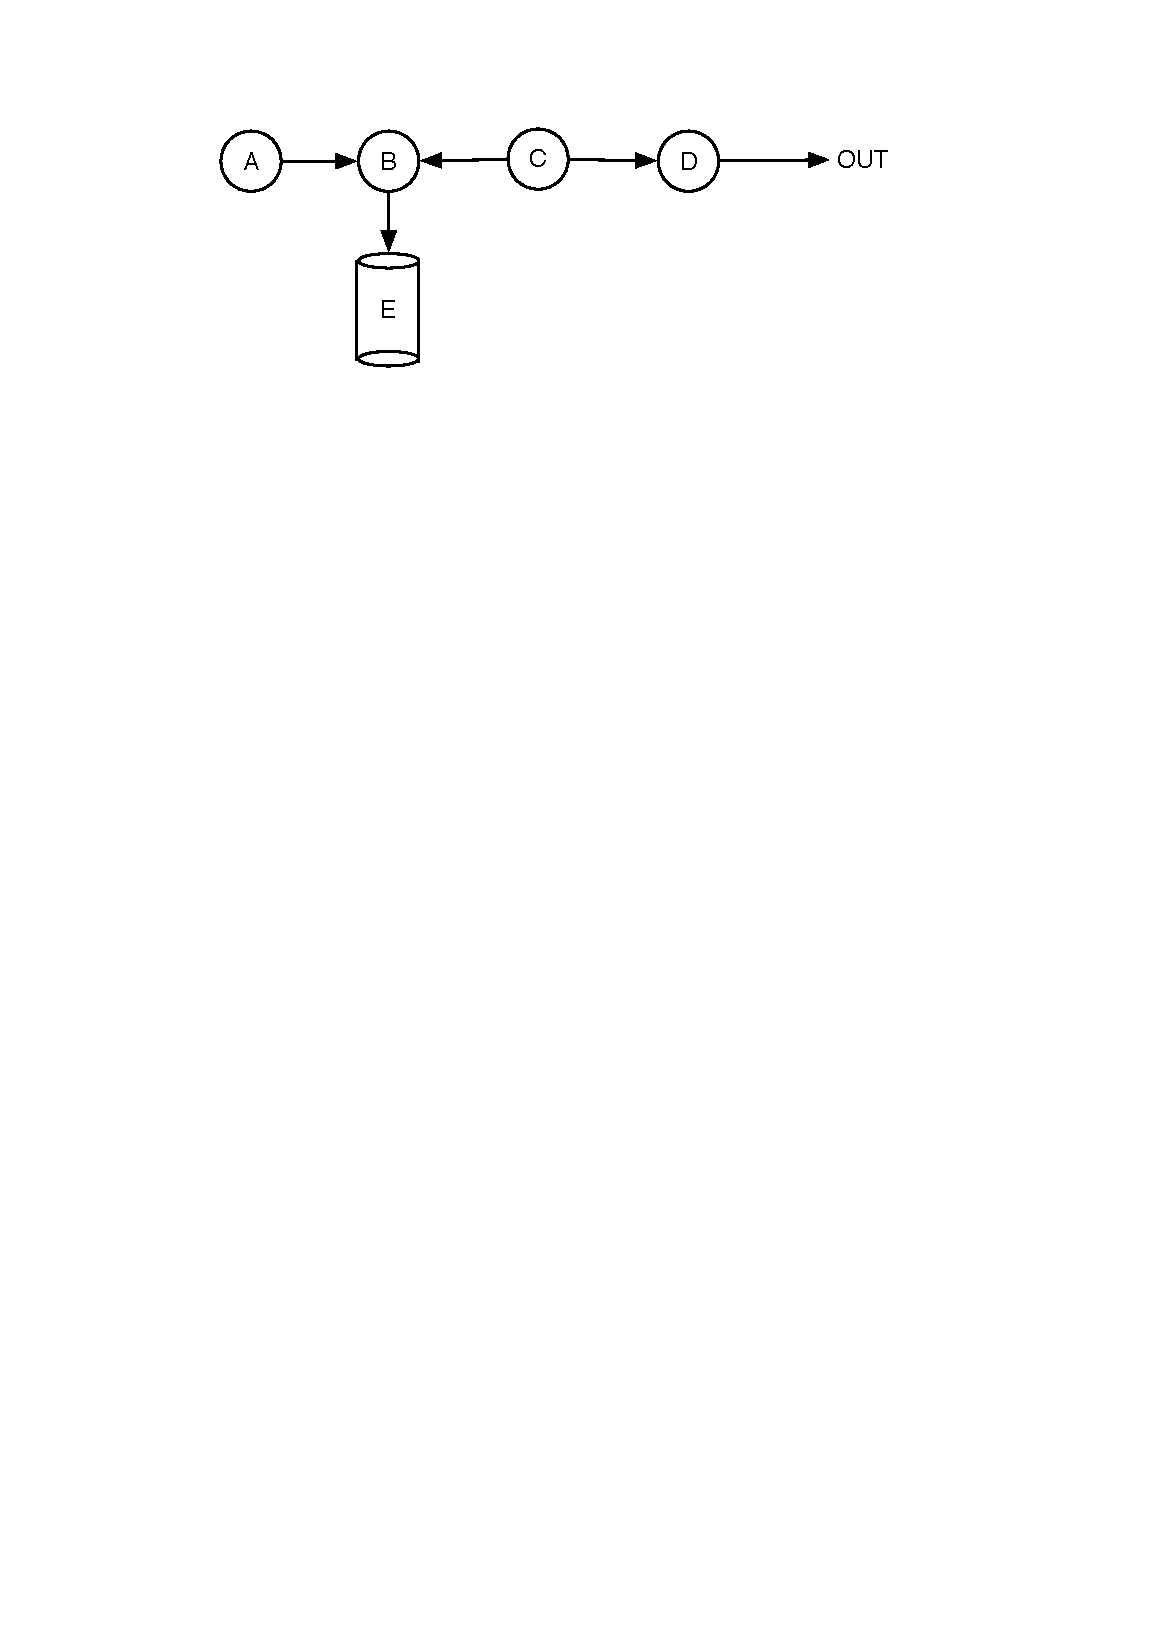
\includegraphics[width=5cm]{images/funnel}
		\caption{funnel.}
		\label{fig:funnel}
	\end{center}
\end{figure}

\subsection{Linearising a topology}

Sorting the processing elements in a topology in a way that topology looks more linear, visually. This step ensures that visual investigation and evaluation of the structural complexity of the topology is possible by direct observation. It is sometimes essential to provide such a visualisation to evaluate how to refactor the topology based on emerging needs.

\begin{figure}[H]
	\begin{center}
		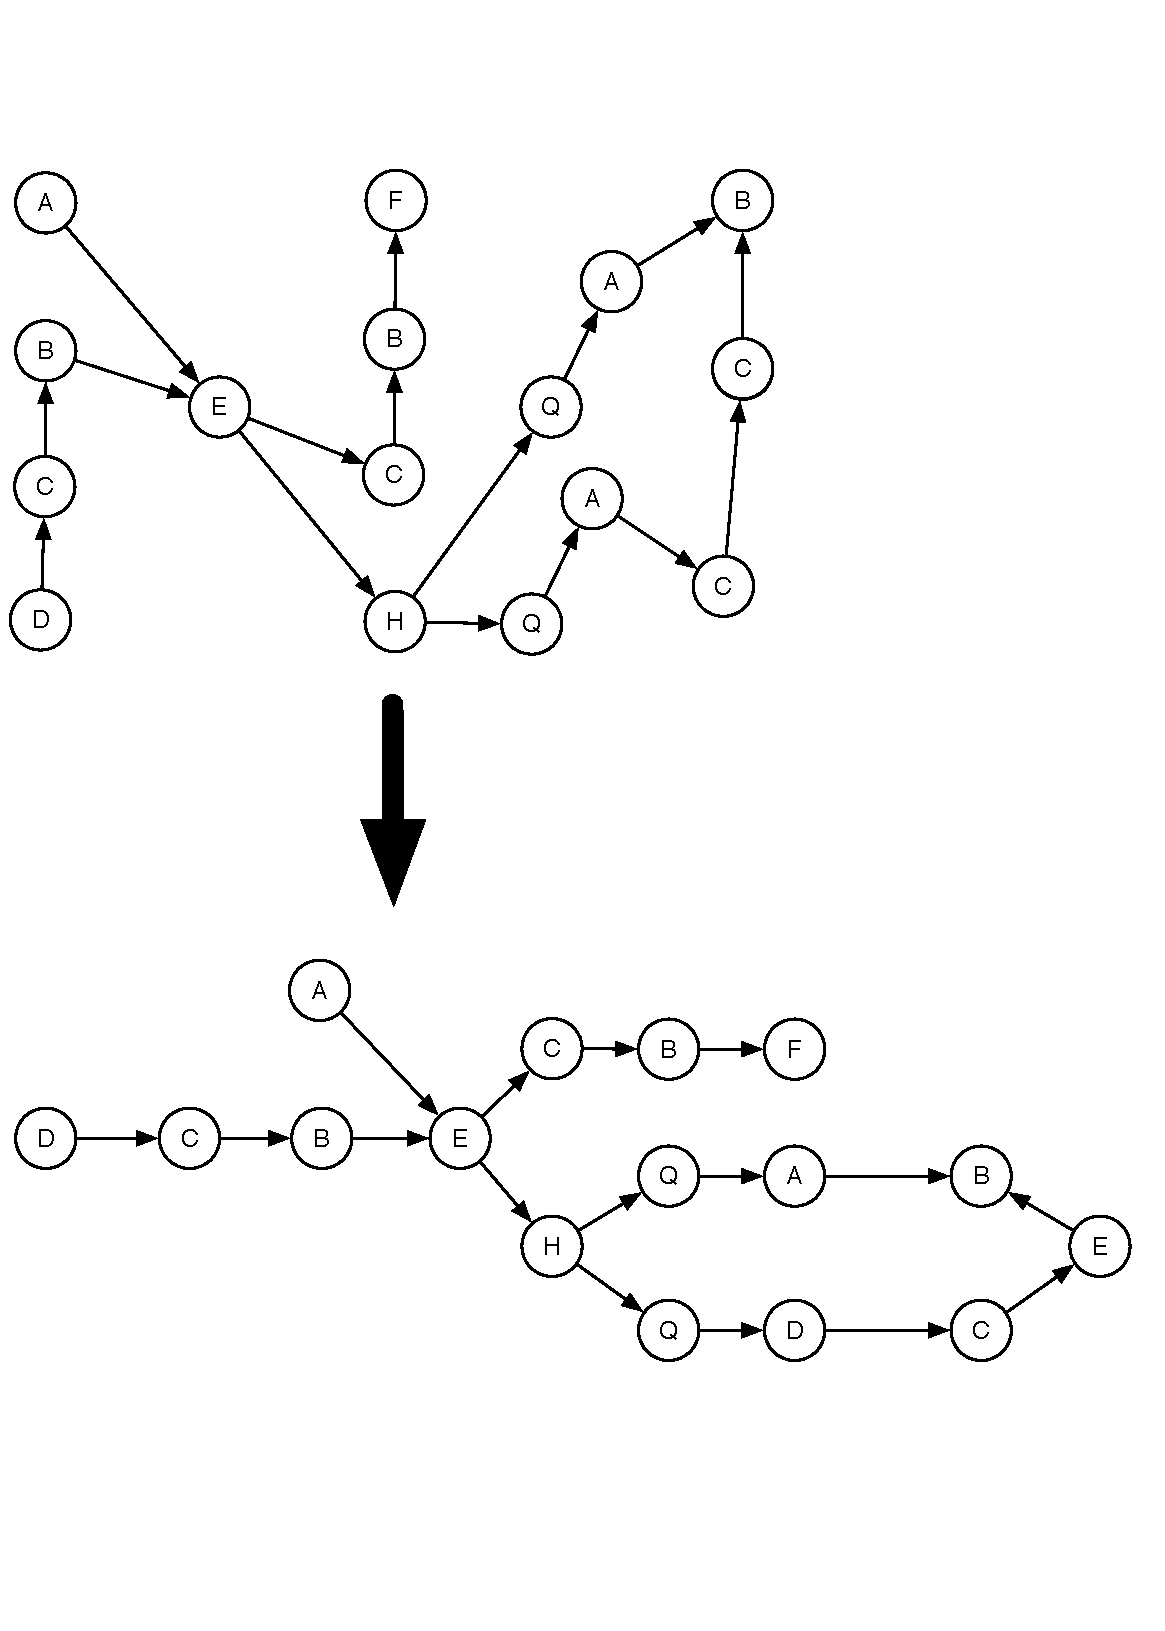
\includegraphics[width=5cm]{images/linearizing}
		\caption{linearizing.}
		\label{fig:linearizing}
	\end{center}
\end{figure}